% !TEX root=../thesis.tex

\chapter{Research Methods} % (fold)
% Research questions and method
\label{cha:research_questions_and_method}
This chapter describes the basic research method used in this 
thesis. We will then describe how the method was used.
\section{Research Methods} % (fold)
\label{sec:research_method}

During the research done in the thesis, we applied the Design Science Research 
Process (DSRP) as the research method. The DSRP is based on 6 steps which are 
presented in the list below. Depending on what the focus of the project is, 
the project can start at almost any of the steps below.\cite{peffers2006design}

\begin{description}
	\item [1. Problem identification and motivation] Defines the problem to be
	researched. 
	\item [2. Objectives of a solution] Infer the goals of the solution.
	\item [3. Design and development] Creates a artifact for the solution.
	\item [4. Demonstration] Demonstrate the created artifact.
	\item [5. Evaluation] Observe and measure how the artifact gives a 
	solution to the problem.
	\item [6. Communication] Communicate the problem along with the artifact.
\end{description}

As Hevner, March, Park, and Ram\cite{von2004design} describes, 
evaluation of a product, produced through a sequence of expert activities 
provides feedback information and a better understanding of the problem in 
order to the quality of the product. By repeating the sequence of expert 
activities means that one have a process loop which is typically iterated a 
number of times before the final design artifact is generated. The process 
loop is demonstrated in \Ref{fig:DSRP}, where one can see the loop as going 
from Step 2 (Objectives of a solution) to Step 5 (Evaluation) and back.\\

By putting together a focus group, one can utilize stakeholders to define the
objectives of a solution. As Nielsen\cite{FocusGroupstoStudyWorkPractice} says,
focus groups can be a great way to learn about the work that occurs "between"
and "around" the solutions. By bringing together several users, one is often 
able to bring out users' spontaneous reactions and ideas\cite{nielsen1997use}.
To ensure that these focus groups stays focused during the entire workshops,
the moderator have to make sure the groups discusses a preplanned set of issues
and set goals for the kind of information to be gathered.


\begin{figure}[!htbp]
	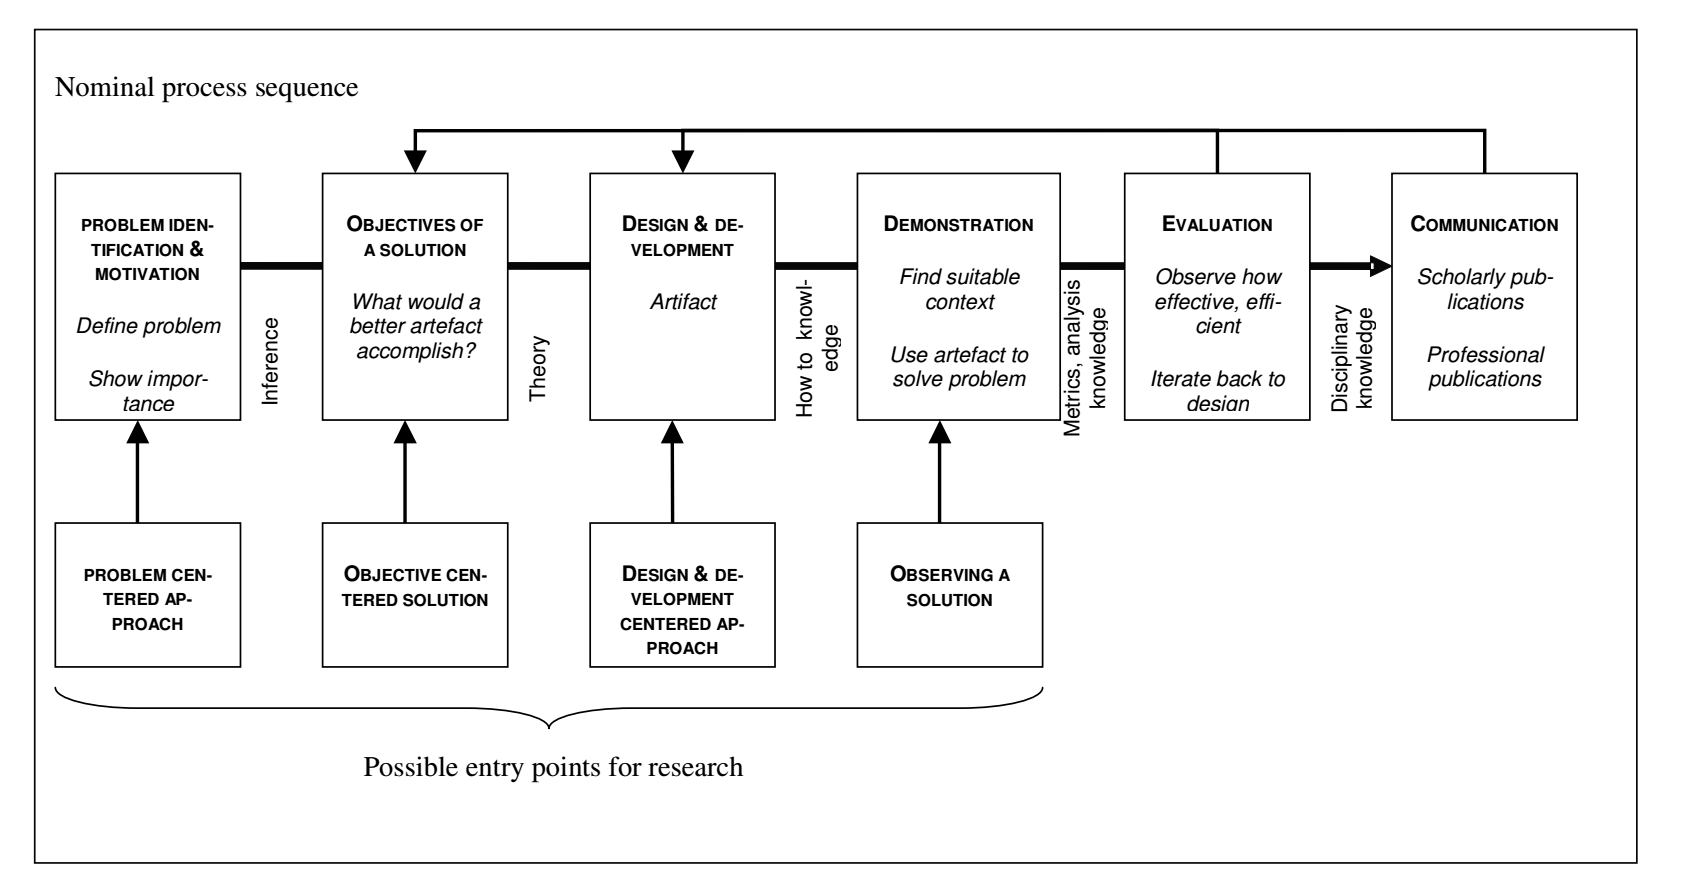
\includegraphics[width=\textwidth,center]{dsrp_modell.png}
	\caption[Design science research process (DSRP) model]{Design research process (DSRP)
	model\cite{peffers2006design}}
	\label{fig:DSRP}
\end{figure}


% section research_method (end)

\section{Project Research} % (fold)
\label{sec:workshops}
In this thesis, the problem was 
identified and motivated prior to the thesis, thus the natural starting 
point of this research was to go into the second stage called objective 
centered. \Ref{fig:DSRP} shows four entry points into a design 
research process; Problem centered-, objective centered-, design\&development-
centered-approach and observing a solution. This thesis was an interaction 
between objectives of a solution, and a study of prior art.

Examining the state-of-the-art and existing systems is done by searching for
scientific articles and commercial systems which contribute towards the goal 
of the thesis and has been performed as a part of the background study. By 
describing these systems and categorizing them, one is able to detect holes in 
available functionality, and in turn comparing the functionality provided by 
the systems against the stakeholders, one can define help define the 
objectives of the solution. \\

%TODO forklar hvordan gjør en elicitation
Since the part of determining the needs and requirements of the stakeholders 
are a important deal of having a stakeholder aware system, it is important to
define these, such as by doing a requirements elicitation. To help define both 
which stakeholders were relevant for the system to beware of, and the needs of 
these stakeholders, a focus groups was put together and met for a discussion
during a workshop. As Goguen and Linde \cite{goguen1993techniques} says, such 
groups have a claim to greatly accelerate the development of requirements.

By having these discussions, one is able to help define specifications for the
system and define the domain. As Zave and Jackson \cite{zave1997four} 
conclude, by among others, have each requirement validated as acceptable to 
the user, and the specifications do not constrain the environment, we are 
guaranteed that if the specification is implemented as an artifact which
is connected to the environment, the requirements will be satisfied. \\

%TODO fyll ut mer
As part of the iterative loop, a meeting with the supervisors were held each 
week. During these meetings the current status of both the case study and
development of the prototype was demonstrated. Based on these demonstrations,
an evaluation of the objectives and the design were performed, and they were
redefined. The process then returned to step 2 or 3, and the the steps forward
were executed again until the we reached the final step, which is the
communication through this thesis.

% section workshops (end)

% chapter research_questions_and_method (end)

